% Modified based on Xiaoming Sun's template
\documentclass{article}
\usepackage{amsmath,amsfonts,amsthm,amssymb}
\usepackage{setspace}
\usepackage{fancyhdr}
\usepackage{lastpage}
\usepackage{extramarks}
\usepackage{chngpage}
\usepackage{soul,color}
\usepackage{graphicx,float,wrapfig}

\usepackage{hyperref}
\hypersetup{
    colorlinks=true,
    linkcolor=blue,
    filecolor=magenta,      
    urlcolor=cyan,
}

\newcommand{\Class}{Mathematics for Computer Science}

% Homework Specific Information. Change it to your own
\newcommand{\Title}{Homework 1}

% In case you need to adjust margins:
\topmargin=-0.45in      %
\evensidemargin=0in     %
\oddsidemargin=0in      %
\textwidth=6.5in        %
\textheight=9.0in       %
\headsep=0.25in         %

% Setup the header and footer
\pagestyle{fancy}                                                       %
\chead{\Title}  %
\rhead{\firstxmark}                                                     %
\lfoot{\lastxmark}                                                      %
\cfoot{}                                                                %
\rfoot{Page\ \thepage\ of\ \protect\pageref{LastPage}}                          %
\renewcommand\headrulewidth{0.4pt}                                      %
\renewcommand\footrulewidth{0.4pt}                                      %

%%%%%%%%%%%%%%%%%%%%%%%%%%%%%%%%%%%%%%%%%%%%%%%%%%%%%%%%%%%%%
% Some tools
\newcommand{\enterProblemHeader}[1]{\nobreak\extramarks{#1}{#1 continued on next page\ldots}\nobreak%
                                    \nobreak\extramarks{#1 (continued)}{#1 continued on next page\ldots}\nobreak}%
\newcommand{\exitProblemHeader}[1]{\nobreak\extramarks{#1 (continued)}{#1 continued on next page\ldots}\nobreak%
                                   \nobreak\extramarks{#1}{}\nobreak}%

\newcommand{\homeworkProblemName}{}%
\newcounter{homeworkProblemCounter}%
\newenvironment{homeworkProblem}[1][Problem \arabic{homeworkProblemCounter}]%
  {\stepcounter{homeworkProblemCounter}%
   \renewcommand{\homeworkProblemName}{#1}%
   \section*{\homeworkProblemName}%
   \enterProblemHeader{\homeworkProblemName}}%
  {\exitProblemHeader{\homeworkProblemName}}%

\newcommand{\homeworkSectionName}{}%
\newlength{\homeworkSectionLabelLength}{}%
\newenvironment{homeworkSection}[1]%
  {% We put this space here to make sure we're not connected to the above.

   \renewcommand{\homeworkSectionName}{#1}%
   \settowidth{\homeworkSectionLabelLength}{\homeworkSectionName}%
   \addtolength{\homeworkSectionLabelLength}{0.25in}%
   \changetext{}{-\homeworkSectionLabelLength}{}{}{}%
   \subsection*{\homeworkSectionName}%
   \enterProblemHeader{\homeworkProblemName\ [\homeworkSectionName]}}%
  {\enterProblemHeader{\homeworkProblemName}%

   % We put the blank space above in order to make sure this margin
   % change doesn't happen too soon.
   \changetext{}{+\homeworkSectionLabelLength}{}{}{}}%

\newcommand{\Answer}{\ \\\textbf{Answer:} }
\newcommand{\Acknowledgement}[1]{\ \\{\bf Acknowledgement:} #1}

%%%%%%%%%%%%%%%%%%%%%%%%%%%%%%%%%%%%%%%%%%%%%%%%%%%%%%%%%%%%%


%%%%%%%%%%%%%%%%%%%%%%%%%%%%%%%%%%%%%%%%%%%%%%%%%%%%%%%%%%%%%
% Make title
\title{\textmd{\bf \Class: \Title}}
\date{March 1, 2019}
\author{Xingyu Su 2015010697}
%%%%%%%%%%%%%%%%%%%%%%%%%%%%%%%%%%%%%%%%%%%%%%%%%%%%%%%%%%%%%

\begin{document}
\begin{spacing}{1.1}
\maketitle \thispagestyle{empty}

%%%%%%%%%%%%%%%%%%%%%%%%%%%%%%%%%%%%%%%%%%%%%%%%%%%%%%%%%%%%%
% Begin edit from here

%%%%%%%%%%%%%%%%%%%%%%%%%%%%%%%%%%%%%%%%%%%%%%%%%%%%%%%%%%%%%
% HOMEWORK-1-LPV 1.8.26
\begin{homeworkProblem}[LPV 1.8.26]
Find the number of all 20-digit integers in which no two consecutive digits are the same.

\Answer 

The first digit has 0-9 ten choices, and the second will have only 9 choices left because it can not be the same with the first digit. So as all the left 18-digits. As a result, the answer should be:

$10 \cdot 9^{19} = 1441151880758558720 \approx 1.44\times10^{18} $

\end{homeworkProblem}
%%%%%%%%%%%%%%%%%%%%%%%%%%%%%%%%%%%%%%%%%%%%%%%%%%%%%%%%%%%%%


%%%%%%%%%%%%%%%%%%%%%%%%%%%%%%%%%%%%%%%%%%%%%%%%%%%%%%%%%%%%%
% HOMEWORK-1-LPV 1.8.29
\begin{homeworkProblem}[LPV 1.8.29]
What is the number of ways to color n objects with 3 colors if every color must be used at least once?

\Answer

For the case of $n<2$, obviously the answer is 0, and when $n = 3$, answer is 1. Considering a big n, the answer should be equal to the permutations of choosing any color of 3 for any object substract the permutations of choosing any 2 colors of 3 for any object.

Generally, The answer $ans$ is:

    \hspace{1em} if $n<2$, $ans=0$

    \hspace{1em} if $n \geq 3$, $ans=\binom{3}{3} \times 3^n - \binom{3}{2}\times 2^n$ 

\end{homeworkProblem}
%%%%%%%%%%%%%%%%%%%%%%%%%%%%%%%%%%%%%%%%%%%%%%%%%%%%%%%%%%%%%


%%%%%%%%%%%%%%%%%%%%%%%%%%%%%%%%%%%%%%%%%%%%%%%%%%%%%%%%%%%%%
% HOMEWORK-1-LPV 2.1.8
\begin{homeworkProblem}[LPV 2.1.8]
Prove that the sum of the first $n$ squares $1+4+9+\cdots+n^2$ is $n(n+1)(2n+1)/6.$

\Answer

Consider $n=1$, we have $1=1*(1+1)*(2*1+1)/6$, so the equation is proved to be true when $n=1$.

Consider the equation is true when $n=k$, then we have:

\hspace{1em}
$\sum_{i=1}^{k+1}{i^2}
=\sum_{i=1}^k{i^2}+(k+1)^2
=\frac{k(k+1)(2k+1)}{6}+(k+1)^2
=\frac{(k+1)[2k^2+k+6(k+1)]}{6}
=\frac{(k+1)(k+2)(2k+3)}{6}
$

which means $\sum_{i=1}^{n}{i^2}=\frac{n(n+1)(2n+1)}{6}$ is true when $n=k+1$.

So the equation is true for all positive numbers $n=1, 2, 3, \cdots$

\end{homeworkProblem}
%%%%%%%%%%%%%%%%%%%%%%%%%%%%%%%%%%%%%%%%%%%%%%%%%%%%%%%%%%%%%


%%%%%%%%%%%%%%%%%%%%%%%%%%%%%%%%%%%%%%%%%%%%%%%%%%%%%%%%%%%%%
% HOMEWORK-1-LPV 2.1.13
\begin{homeworkProblem}[LPV 2.1.13]
Read carefully the following induction proof:

Assertion: Balabala...

Proof: Balabala...

But the assertion we proved is clearly wrong; where is the error?

\Answer

Because the \textbf{Proof} part used more than 2 lines, but the induction part can only prove the \textbf{Assertion} is true when there are two lines.

\end{homeworkProblem}
%%%%%%%%%%%%%%%%%%%%%%%%%%%%%%%%%%%%%%%%%%%%%%%%%%%%%%%%%%%%%


%%%%%%%%%%%%%%%%%%%%%%%%%%%%%%%%%%%%%%%%%%%%%%%%%%%%%%%%%%%%%
% HOMEWORK-1-LPV 2.5.2
\begin{homeworkProblem}[LPV 2.5.2]
What is the following sum?

$0 \cdot \binom{n}{0} + 1 \cdot \binom{n}{1} + 2 \cdot \binom{n}{2} + \cdots + (n-1) \cdot \binom{n}{n-1} + n \cdot \binom{n}{n}$

Experiment, conjecture the value, and then prove it. (Try to prove the result by induction and also by combinatorial arguments.)

\Answer

Denote the sum of the equation as $f(n)$, and do experiments for $n=1,2,3,4,5$, we can get:

\hspace{1em} $n=1$, $f(1)=0+1=1=1 \times 2^0$

\hspace{1em} $n=2$, $f(2)=0+1 \times 2+2 \times 1=4=2 \times 2^1$

\hspace{1em} $n=3$, $f(3)=0+1 \times 3+2 \times 3+3 \times 1=12=3 \times 2^2$

\hspace{1em} $n=4$, $f(4)=0+1 \times 4+2 \times 6+3 \times 4+4 \times 1=32=4 \times 2^3$

\hspace{1em} $n=5$, $f(5)=0+1 \times 5+2 \times 10+3 \times 10+4 \times 5+5 \times 1=80=5 \times 2^4$

From induction, we can guess when $n=k$, $f(k)=k\times 2^{k-1}$. And here we can get:

\hspace{1em} $\binom{n}{m} = \binom{n-1}{m-1} \times n / m$

\hspace{1em} $m \binom{n}{m} = \binom{n-1}{m-1}\times n$

So:

\hspace{1em} $\sum_{m=1}^n m \binom{n}{m} = \sum_{m=1}^n (\binom{n-1}{m-1} \times n) =  n \times \sum_{m=0}^{n-1} \binom{n}{m} = n 2^{n-1}$

\end{homeworkProblem}
%%%%%%%%%%%%%%%%%%%%%%%%%%%%%%%%%%%%%%%%%%%%%%%%%%%%%%%%%%%%%


%%%%%%%%%%%%%%%%%%%%%%%%%%%%%%%%%%%%%%%%%%%%%%%%%%%%%%%%%%%%%
% HOMEWORK-1-LPV 2.5.7
\begin{homeworkProblem}[LPV 2.5.7]

We select 38 even positive integers, all less than 1000. Prove that there will be two of them whose difference is at most 26.

\Answer 

If every each two numbers' difference is bigger than 26, consider the fisrt number is 2, then the next is at least 29, which in result should be 30. With this strategy, after choosing the first 38 even positive integers, we will get 2, 30, ... , 1010, 1038. So smallest difference between any 2 numbers should be smaller than 28.

If every each two numbers' difference is no smaller than 26, consider the fisrt number is 2, then the next is at least 27, which in result should be 28. With this strategy, after choosing the first 38 even positive integers, we will get 2, 28, ... , 938, 964. So smallest difference between any 2 numbers is 26.

\end{homeworkProblem}
%%%%%%%%%%%%%%%%%%%%%%%%%%%%%%%%%%%%%%%%%%%%%%%%%%%%%%%%%%%%%


%%%%%%%%%%%%%%%%%%%%%%%%%%%%%%%%%%%%%%%%%%%%%%%%%%%%%%%%%%%%%
% HOMEWORK-1-Special Problem 1
\begin{homeworkProblem}[Special Problem 1]
\hspace{1em} 
(a) In the birthday problem discussed in class (with 72 students present), using the same probability space, let $T_1$ be the event that there is a triple-collision, i.e. three students having the same birthday. Calculate the numerical value of $Pr\{T_1\}$.

(b) In the same probability space as above, let $T_2$ be the event that there are at least 6 disjoint same-birthday pairs of students. Calculate the numerical value of $Pr\{T_2\}$.

\Answer 

(a) Consider the opposite conditions, we can get all events count as below:

\hspace{1em}
$|\Omega| - |T_1| = A^{72}_{366}+C^{2}_{72}A^{71}_{366}+C^{2}_{72}C^{2}_{70}A^{70}_{366}/{2!}+\cdots+C^{2}_{72}C^{2}_{70}\cdots C^{2}_{2}A^{36}_{366}/{36!}$

\hspace{1em}
$Pr\{T_1\} = 1 - |T_1|/|\Omega| = 1-\frac{1}{366^{72}}(\frac{1}{2^0 0!}A^{72}_{366}+\frac{1}{2^1 1!}A^{2}_{72}A^{71}_{366}+\frac{1}{2^2 2!}A^{4}_{72}A^{70}_{366}+\cdots+\frac{1}{2^{36} 36!}A^{72}_{72}A^{36}_{366})$

Which is found true in (2) of \href{https://ac.els-cdn.com/S0378375804002721/1-s2.0-S0378375804002721-main.pdf?_tid=7580fe67-40c2-467b-8487-b348cae793a5&acdnat=1551672820_3458fd64ec45ba9465eb28ddba80e341}{doi:10.1016/j.jspi.2003.11.015}:  %DevSkim: ignore DS173237 

\hspace{1em}
$Pr\{T_1\} = 1 - \sum_{i=0}^{[n/2]}{\frac{m!n!}{i!(n-2i)!(m-n+i)!2^im^n}}$

The result is calculated to be $Pr\{T_1\}=0.3267$. And Figure 1 shows the probability of triple-collision with number of students varies from 10 to 100.

\begin{figure}[h]
  \centering
  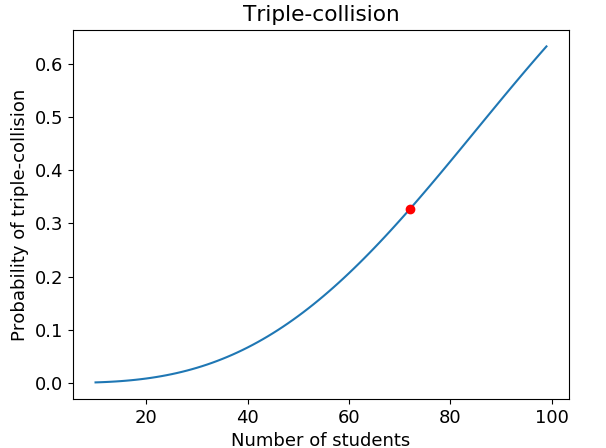
\includegraphics[width=0.6\linewidth]{figures/hw1_fig1}
  \caption{Probability of triple-collision with number of students varies from 10 to 100.}
  \label{fig:triple-collision}
\end{figure}

(b) The conditions are very hard and after hours thinking I gived it up. But a statistic counting is done by `python' as shown in Figure 2, from which the result is $Pr\{T_2\} \approx 0.0612$

\begin{figure}[h]
  \centering
  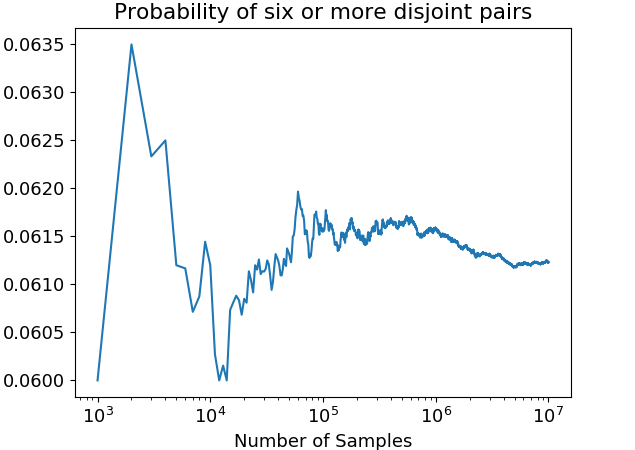
\includegraphics[width=0.6\linewidth]{figures/hw1_fig2}
  \caption{Probability of six or more disjoint pairs}
  \label{fig:six-disjoint}
\end{figure}

\end{homeworkProblem}
%%%%%%%%%%%%%%%%%%%%%%%%%%%%%%%%%%%%%%%%%%%%%%%%%%%%%%%%%%%%%


%%%%%%%%%%%%%%%%%%%%%%%%%%%%%%%%%%%%%%%%%%%%%%%%%%%%%%%%%%%%%
% HOMEWORK-1-Special Problem 2
\begin{homeworkProblem}[Special Problem 2]

\hspace{1em}
(a) Develop a mathematical probability model for the Monte Hall Problem discussed in class. Specify mathematically the events corresponding, respectively, to the success of the strategies Switch and No-Switch. Show that $Pr\{No\ Switch\} = 1/3$, and $Pr\{Switch\} = 2/3$.

(b) Suppose Host Monte Hall puts the coveted car behind doors 1, 2, 3 with probabilities 1/2, 1/3, 1/6 respectively (instead of uniformly as in class). Assume the contestant initially picks door 1. How should you modify your probability space? What is the value of $Pr\{No\ Switch\}$ and $Pr\{Switch\}$.

\Answer 

(a) It's easy to denote three doors to be 1, 2, 3 with probalibities 1/3, 1/3, 1/3 respectively. Assume the contestant initially picks door 1. So with initial guess:

\hspace{1em}
$Pr\{car\ in\ 1\} = 1/3$, $Pr\{car\ in\ 2\ or\ 3\} = 2/3$

We can know that conditional probabilities is:

\hspace{1em}
$Pr\{Switch\} = Pr(Switch\ win | car\ in\ 1) + Pr(Switch\ win | car\ in\ 2\ or\ 3) = Pr\{car\ in\ 1\} \times 0+Pr\{car\ in\ 2\ or\ 3\} \times 1 = 1/3 \times 0 + 2/3 \times 1 = 2/3 $

\hspace{1em}
$Pr\{No\ Switch\} = Pr(No\ Switch\ win | car\ in\ 1) + Pr(No\ Switch\ win | car\ in\ 2\ or\ 3) = Pr\{car\ in\ 1\} \times 1 + Pr\{car\ in\ 2\ or\ 3\} \times 0 = 1/3 \times 1 + 2/3 \times 0 = 1/3 $


(b) Similarly to (a), we can get:

\hspace{1em}
$Pr\{car\ in\ 1\} = 1/2$, $Pr\{car\ in\ 2\ or\ 3\} = 1/2$

So we can know that conditional probabilities is:

\hspace{1em}
$Pr\{Switch\} = Pr(Switch\ win | car\ in\ 1) + Pr(Switch\ win | car\ in\ 2\ or\ 3) = Pr\{car\ in\ 1\} \times 0+Pr\{car\ in\ 2\ or\ 3\} \times 1 = 1/2 \times 0 + 1/2 \times 1 = 1/2 $

\hspace{1em}
$Pr\{No\ Switch\} = Pr(No\ Switch\ win | car\ in\ 1) + Pr(No\ Switch\ win | car\ in\ 2\ or\ 3) = Pr\{car\ in\ 1\} \times 1 + Pr\{car\ in\ 2\ or\ 3\} \times 0 = 1/2 \times 1 + 1/2 \times 0 = 1/2 $

\end{homeworkProblem}
%%%%%%%%%%%%%%%%%%%%%%%%%%%%%%%%%%%%%%%%%%%%%%%%%%%%%%%%%%%%%


%%%%%%%%%%%%%%%%%%%%%%%%%%%%%%%%%%%%%%%%%%%%%%%%%%%%%%%%%%%%%
% HOMEWORK-1-Special Problem 3
\begin{homeworkProblem}[Special Problem 3]

\hspace{1em}
A 4 by 4 box is filled with integers 1,2,...,15 with the lower right corner initially left empty. (See the figure on next page.) At any time there is exactly one cell empty. At each step you may move to the empty cell one of its adjacent number. Question: Prove that the second configuration cannot be reached from the first configuration.

\begin{figure}[h]
  \centering
  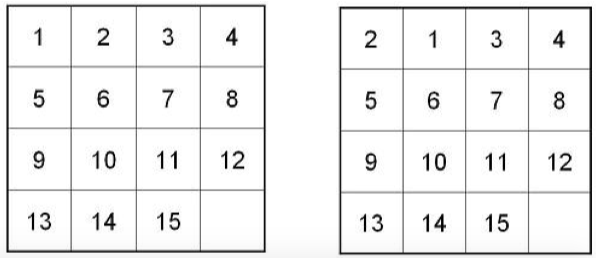
\includegraphics[width=0.5\linewidth]{figures/hw1_fig3}
  \caption{4 by 4 box for Special Problem 3.}
  \label{fig:boxes}
\end{figure}

\Answer 

There are to truth easy to be found:

\hspace{1em}
(1) When the blank box moves around and returns to it's original position, the number of it's moves must be even.

\hspace{1em}
(2) Denote one set of box values as one state (blank can be denote as 0 or any number bigger than 15). If after $m$ times of value changes, state \textbf{a} turns to be state \textbf{b}. Then for any route from state \textbf{a} to state \textbf{b}, the number of value changes $n$ must have relationship with $m$:

\hspace{2em}
$mod(|m-n|,2) = 0$

Denote left box matrix as state $s_1$, right box matrix as state $s_2$. Using truth (1), the number of moves of blank must be even number. But with truth (2), the moves between $s_1$ and $s_2$ must be odd number. The conflict reveals that $s_2$ cannot be reached by $s_1$.

\end{homeworkProblem}
%%%%%%%%%%%%%%%%%%%%%%%%%%%%%%%%%%%%%%%%%%%%%%%%%%%%%%%%%%%%%


% ACKNOWLEGEMENT
\Acknowledgement{

[1] Thanks to \href{https://en.wikipedia.org/wiki/Birthday_problem}{Wikipedia: Birthday problem} and \href{https://ac.els-cdn.com/S0378375804002721/1-s2.0-S0378375804002721-main.pdf?_tid=7580fe67-40c2-467b-8487-b348cae793a5&acdnat=1551672820_3458fd64ec45ba9465eb28ddba80e341}{doi:10.1016/j.jspi.2003.11.015} for SP1(a) % DevSkim: ignore DS173237 

}

% End edit to here
%%%%%%%%%%%%%%%%%%%%%%%%%%%%%%%%%%%%%%%%%%%%%%%%%%%%%%%%%%%%%

\end{spacing}
\end{document}

%%%%%%%%%%%%%%%%%%%%%%%%%%%%%%%%%%%%%%%%%%%%%%%%%%%%%%%%%%%%%
